\documentclass{article}
\usepackage{amsmath}
\usepackage{amssymb}
\usepackage{graphicx}
\usepackage{tikz}
\usetikzlibrary{arrows}
\usepackage{verbatim}
\usepackage{psfrag}
\usepackage{here} 
\usepackage{hyperref}
\usepackage{xcolor}
\usepackage{tcolorbox}
\usepackage{geometry}

 \geometry{
 a4paper,
 total={150mm,257mm},
 left=30mm,
 top=20mm,
 }

\renewcommand{\familydefault}{\sfdefault}
\renewcommand{\familydefault}{cmss}

\begin{document}

\begin{center}
\bf{\large 
{\Large Aprendizaje Autom\'atico}\\
{\vspace{0.1cm}}
Pr\'actica 1
}
\end{center}

\bigskip

\begin{itemize}

\item[1)]  {\bf An\'alisis exploratorio de los datos}

Importa los datos del fichero \texttt{dataset.csv} y realiza el an\'alisis exploratorio de los datos. Describe en el informe los resultados de este análisis y deposita el c\'odigo Python en Aula Virtual en el fichero \texttt{answer1.ipynb}.

\end{itemize}

\bigskip

\begin{itemize}

\item[2)] {\bf Clasificaci\'on usando todas las caracter\'{\i}sticas de los datos}

Usando todas las caracter\'{\i}sticas, implementa los m\'etodos 

\begin{itemize}

\item
Logistic Regression, 

\item
SVM, y

\item
Random Trees

\end{itemize}

para clasificar los datos. Describe en el informe los par\'ametros usados y los resultados obtenidos con los distintos m\'etodos y deposita el c\'odigo Python en Aula Virtual en el fichero \texttt{answer2.ipynb}.

\end{itemize}

\bigskip

\begin{itemize}

\item[3)] {\bf Clasificaci\'on usando 4 caracter\'{\i}sticas de los datos}

Selecciona 4 caracter\'isticas de los datos. Usando estas caracter\'{\i}sticas, implementa los m\'etodos 

\begin{itemize}

\item
Logistic Regression, 

\item
SVM, y

\item
Random Trees

\end{itemize}

para clasificar los datos. Describe en el informe los par\'ametros usados y los resultados obtenidos con los distintos m\'etodos y deposita el c\'odigo Python en Aula Virtual en el fichero \texttt{answer3.ipynb}.

\end{itemize}

\bigskip

\begin{itemize}

\item[4)] {\bf Clasificaci\'on usando 2 caracter\'{\i}sticas de los datos}

Selecciona 2 caracter\'isticas de los datos. Usando estas caracter\'{\i}sticas, implementa los m\'etodos 

\begin{itemize}

\item
Logistic Regression, 

\item
SVM, y

\item
Random Trees

\end{itemize}

para clasificar los datos. Describe en el informe los par\'ametros usados y los resultados obtenidos con los distintos m\'etodos y deposita el c\'odigo Python en Aula Virtual en el fichero \texttt{answer4.ipynb}.

\end{itemize}

\bigskip

\noindent
\textcolor{red}{
Redacta un informe detallado respondiendo a cada pregunta en una secci\'on diferente. Motiva cada elecci\'on realizada durante el proceso de dise\~no de los clasificadores y describe cada resultado obtenido. Compara los resultados obtenidos con distintos n\'umeros de caracter\'{\i}sticas. Incluye el c\'odigo Python en el apartado correspondiente del informe. 
} 

% ----- 1. ANALISIS EXPLORATORIO DE LOS DATOS ----- %

\newpage

\section[1]{An\'alisis exploratorio de los datos}

\bigskip

\begin{itemize}

\item[1.1]  {\bf Importaci\'on del dataset}

El primer paso de este an\'alisis consiste en la importaci\'on del dataset, utilizando la librer\'ia pandas para leer el fichero \texttt{dataset.csv}. A partir de ah\'i, se configura la visualizaci\'on del dataset para poder observar todas las columnas disponibles.

Este paso es importante para obtener una vista inicial del tamaño y las caracter\'isticas del dataset, ademas de confirmar que los datos han sido le\'idos correctamente.

\begin{tcolorbox}[width=14cm]
\begin{scriptsize}
\begin{verbatim}
dataset = pd.read_csv("dataset.csv")
pd.set_option('display.max_columns', len(dataset.columns))
\end{verbatim}
\end{scriptsize}
\end{tcolorbox}

\end{itemize}

\bigskip

\begin{itemize}

\item[1.2]  {\bf Inspecci\'on del dataset}

A continuaci\'on, se eval\'ua la estructura del dataset observando las dimensiones (dataset.shape), las primeras filas (dataset.head(1)), la informaci\'on de cada columna y otras estad\'isticas descriptivas como la media, la desviaci\'on estandar, m\'inimos, m\'aximos y cuartiles, adem\'as de otros valores at\'ipicos y distribuciones inusuales (dataset.describe()).

Todo esto permite conocer cu\'antas filas y columnas contiene el dataset (dataset.columns), el tipo de datos que maneja (dataset.info()), la aparici\'on de valores nulos o la presencia de inconsistencia en alg\'un dato.

\begin{tcolorbox}[width=14cm]
\begin{scriptsize}
\begin{verbatim}
dataset.columns
dataset.shape
dataset.head(1)
dataset.info()
dataset.describe()
\end{verbatim}
\end{scriptsize}
\end{tcolorbox}

\end{itemize}

\bigskip

\begin{itemize}

\item[1.3]  {\bf Anonimizaci\'on de los datos y an\'alisis de correlaci\'on}

Para poder analizar los datos, se ha creado un nuevo conjunto de datos anonimizado, en el que se ha eliminado la columna \texttt{Target} del dataset. Adem\'as de esto, se realiza un an\'alisis de la correlaci\'on entre todas las variables.

Es importante realizar este paso para detectar altas correlaciones, las cuales suelen indicar multicolinealidad, algo que afecta a los modelos predictivos.

\begin{tcolorbox}[width=14cm]
\begin{scriptsize}
\begin{verbatim}
dataset_anonymized = dataset.drop(["Target"], axis=1)
dataset_anonymized.to_csv('dataset_anonymized.csv', index=False)
dataset_anonymized.corr()
\end{verbatim}
\end{scriptsize}
\end{tcolorbox}

El an\'alisis de una correlacion est\'a identificada con las dem\'as, donde un coeficiente de correlaci\'on cercano a 1 o -1 indica una correlaci\'on fuerte, mientras que un valor cercano a 0 indica una correlaci\'on pr\'acticamente inexistente.

\end{itemize}

\newpage

\begin{itemize}

\item[1.4]  {\bf Visualizaci\'on de la matriz de correlaci\'on}

La matriz de correlaci\'on se visualiza mediante un mapa de calor utilizando la librer\'ia \texttt{seaborn}, la cual facilita la identificaci\'on de relaciones positivas o negativas entre las variables.

\begin{tcolorbox}[width=14cm]
\begin{scriptsize}
\begin{verbatim}
fig, ax = plt.subplots(figsize=(9,9))
sb.heatmap(dataset.corr(), linewidth=0.5, annot=True)
\end{verbatim}
\end{scriptsize}
\end{tcolorbox}

El gr\'afico resultante proporciona una visi\'on m\'as clara de las relaciones m\'as fuertes entre las variables, donde los colores oscuros indican una correlaci\'on alta, mientras que los colores m\'as claros indican una correlaci\'on baja.

\begin{figure}[h]
  \centering
  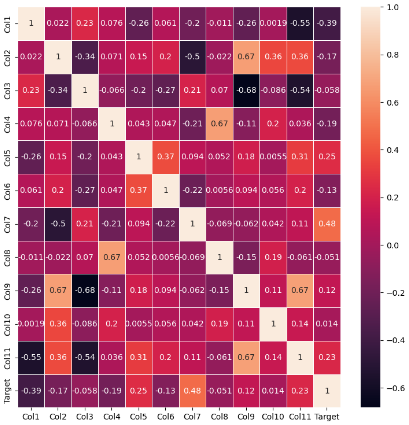
\includegraphics[width=14cm, height=14cm]{correlation_heatmap.png}
\end{figure}

\end{itemize}

\newpage

\begin{itemize}

\item[1.5]  {\bf Visualizaci\'on de distribuciones}

Para observar la distribuci\'on de cada una de las variables en el dataset anonimizado, se generan histogramas que permiten identificar patrones y verificar si las variables est\'an distribuidas de manera normal, poseen sesgos o son valores at\'ipicos.

\begin{tcolorbox}[width=14cm]
\begin{scriptsize}
\begin{verbatim}
columns = dataset_anonymized.columns
fig = plt.figure(figsize=(12,12))
for i in range(0,11):
  ax = plt.subplot(4,4,i+1)
  ax.hist(dataset_anonymized[columns[i]], bins=20, color='blue', edgecolor='black')
  ax.set_title(dataset_anonymized.head(0)[columns[i]].name)
plt.tight_layout()
plt.show()
\end{verbatim}
\end{scriptsize}
\end{tcolorbox}

Estos histogramas muestran la frecuencia de los valores dentro de ciertos intervalos, algo que ayuda a entender mejor la distribuci\'on de los datos.

\begin{figure}[h]
  \centering
  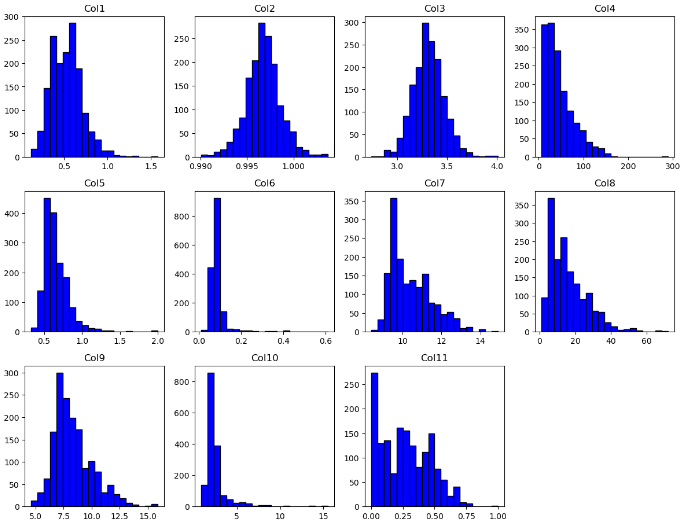
\includegraphics[width=14cm, height=14cm]{characteristics_frequency.png}
\end{figure}

\end{itemize}

\newpage

\begin{itemize}

\item[1.6]  {\bf Separaci\'on de caracter\'isticas y etiquetas}

Una vez hecho esto, se separan las caracter\'isticas (\texttt{X}) y las etiquetas (\texttt{y}) del dataset, lo cual permite preparar los datos para los modelos de Machine Learning.

En este caso, \texttt{X} contiene la informaci\'on de todas las columnas, exceptuando la columna \texttt{Target}, mientras que \texttt{y} contiene los valores de la variable objetivo \texttt{Target}.

\begin{tcolorbox}[width=14cm]
\begin{scriptsize}
\begin{verbatim}
X = dataset_anonymized
y = dataset.get("Target")
print('Class labels:', np.unique(y))

# RESULTADO
Class labels: [3 4 5 6 7 8]
\end{verbatim}
\end{scriptsize}
\end{tcolorbox}

\end{itemize}

\bigskip

\begin{itemize}

\item[1.7]  {\bf Divisi\'on del dataset en entrenamiento y prueba}

El dataset se divide en dos conjuntos: Uno de entrenamiento (0.75) y otro de prueba (0.25). Esta divisi\'on se hace de tal forma que la proporci\'on de clases en ambos conjuntos sea similar, evitando as\'i posibles desbalanceos.

Es necesario realizar este paso para poder entrenar los modelos con una parte del dataset y luego probar su rendimiento con datos que no han sido vistos previamente.

\begin{tcolorbox}[width=14cm]
\begin{scriptsize}
\begin{verbatim}
X_train, X_test, y_train, y_test = train_test_split(X.values, y, test_size=0.25,
 random_state=1, stratify=y)
\end{verbatim}
\end{scriptsize}
\end{tcolorbox}

\end{itemize}

\bigskip

\begin{itemize}

\item[1.8]  {\bf Estandarizaci\'on de los datos}

La estandarizaci\'on de los datos asegura que todas las caracter\'isticas se encuentren en la misma escala, algo que es considerado de gran importancia en modelos de regresi\'on log\'istica, SVM o redes neuronales, los cuales se ver\'an m\'as adelante.

Para este caso, se utiliza StandardScaler() para normalizar los datos, los cuales se ajustan a las caracter\'isticas de los mismos para que tengan media 0 y desviaci\'on est\'andar 1, lo que se traduce en una mejora de rendimiento a la hora de utilizar los algoritmos mencionados anteriormente.

\begin{tcolorbox}[width=14cm]
\begin{scriptsize}
\begin{verbatim}
sc = StandardScaler()
sc.fit(X_train)
X_train_std = sc.transform(X_train)
X_test_std = sc.transform(X_test)
\end{verbatim}
\end{scriptsize}
\end{tcolorbox}

\end{itemize}

\bigskip

\begin{itemize}

\item[1.9]  {\bf Verificaci\'on del balance de clases}

Y por \'ultimo, se eval\'ua el balance de las clases tanto en los datos de entrenamiento como en los datos de prueba para verificar si existe algun tipo de desbalance en las etiquetas, ya que de darse este caso, se podr\'ia producir un desbalance significativo que puede afectar a la capacidad predictiva del modelo.

\begin{tcolorbox}[width=14cm]
\begin{scriptsize}
\begin{verbatim}
print('Labels counts in y:', np.bincount(y))
print('Labels counts in y_train:', np.bincount(y_train))
print('Labels counts in y_test:', np.bincount(y_test))

# RESULTADO
Labels counts in y:       [  0   0   0  10  53  681   638   199   18  ]
Labels counts in y_train: [  0   0   0   8  40  511   478   149   13  ]
Labels counts in y_test:  [  0   0   0   2  13  170   160    50    5  ]
\end{verbatim}
\end{scriptsize}
\end{tcolorbox}

Es importante mencionar que el balance de clases da una idea de si existe predominancia de una clase sobre otra, algo que podr\'ia requerir de t\'ecnicas de remuestreo para mitigar el sesgo.

\end{itemize}

% ----- 2. CLASIFICACION USANDO TODAS LAS CARACTERISTICAS DE LOS DATOS ----- %

\newpage

\section[2]{Clasificaci\'on usando todas las caracter\'{\i}sticas de los datos}

\bigskip

\begin{itemize}

\item[2.1]  {\bf Introducci\'on}

En este apartado se presentan los resultados de la clasificaci\'on del conjunto de datos del fichero \texttt{dataset.csv} utilizando 3 m\'etodos de aprendizaje supervisado: Regresi\'on Logistica (Logistic Regression), M\'aquinas de Soporte Vectorial (SVM) y \'Arboles de Decisi\'on (Random Trees).

Cada uno de estos clasificadores ha sido entrenado usando todas las caracter\'isticas del dataset. A continuacion, se ir\'an describiendo los par\'ametros utilizados para cada modelo, presentando los resultados obtenidos y discutiendo el rendimiento de cada clasificador.

\end{itemize}

\bigskip

\begin{itemize}

\item[2.2]  {\bf Carga y preparaci\'on de los datos}

Antes de entrenar los modelos, primero se debe cargar el dataset, la anonimizaci\'on de las caracter\'isticas y la separaci\'on de las caracter\'isticas (\texttt{X}) respecto a la etiqueta objetivo (\texttt{y}). 

Adem\'as de esto, tambi\'en se realiza una estandarizaci\'on de las caracter\'isticas, algo que es muy importante realizar para modelos como la Regresi\'on Log\'istica (Logistic Regression) y SVM (Support Vector Machines), que son sensibles a las escalas de las variables.

\begin{tcolorbox}[width=14cm]
\begin{scriptsize}
\begin{verbatim}
dataset = pd.read_csv("dataset.csv")
dataset_all_characteristics = dataset.drop(["Target"], axis=1)
X = dataset_all_characteristics
y = dataset.get("Target")

X_train, X_test, y_train, y_test = train_test_split(X.values, y, test_size=0.25, 
random_state=1, stratify=y)
sc = StandardScaler()
sc.fit(X_train)
X_train_std = sc.transform(X_train)
X_test_std = sc.transform(X_test)
\end{verbatim}
\end{scriptsize}
\end{tcolorbox}

Por otro lado, el dataset se divide en dos conjuntos: Uno de entrenamiento (0.75) y otro de prueba (0.25). Esta divisi\'on se hace de tal forma que la proporcion de clases en ambos conjuntos sea similar, evitando as\'i posibles desbalanceos.

\end{itemize}

\bigskip

\begin{itemize}

\item[2.3]  {\bf Regresi\'on Log\'istica (Logistic Regression)}

La Regresi\'on Log\'istica es un modelo lineal, por lo que es m\'as adecuado cuando las caracter\'isticas tienen relaciones lineales con las etiquetas. En este caso, el modelo muestra un buen rendimiento general, aunque la precisi\'on podr\'ia mejorar utilizando t\'ecnicas de selecci\'on de caracter\'isticas o ajustando m\'as los par\'ametros.

A continuaci\'on, se explican brevemente los par\'ametros utilizados:

\begin{itemize}

\item
C = 100.0: El par\'ametro de regularizaci\'on C controla la penalizaci\'on aplicada a los errores. Un valor alto de C indica que se permite una menor penalizaci\'on, por lo que el modelo intenta ajustar m\'as los datos.

\item
solver = 'lbfgs': El solver 'lbfgs' es un optimizador recomendado para solucionar problemas pequeños y medianos.

\item
multi-class = 'ovr': Procedente de las siglas OnevsRest (OVR), significa que para la
clasificaci\'on multiclase, el modelo entrenara un clasificador independiente para cada clase.

\end{itemize}

\begin{tcolorbox}[width=14cm]
\begin{scriptsize}
\begin{verbatim}
lr = LogisticRegression(C=100.0, solver='lbfgs', multi_class='ovr')
lr.fit(X_train_std, y_train)
y_pred = lr.predict(X_test_std)
print('Misclassification samples: %d' % (y_test != y_pred).sum())
print('Accuracy: %.3f' % lr.score(X_test_std, y_test))
\end{verbatim}
\end{scriptsize}
\end{tcolorbox}

Se han obtenido como resultado 165 muestras mal clasificadas, un n\'umero relativamente bajo para este modelo, y una precisi\'on de 0.588, por lo que esa proporci\'on de  predicciones del modelo es correcta.

\end{itemize}

\bigskip

\begin{itemize}

\item[2.4]  {\bf Maquinas de Soporte Vectorial (SVM)}

El SVM con kernel RBF es potente en la captura de relaciones no lineales entre las caracter\'isticas. El modelo muestra un rendimiento s\'olido y, aunque los resultados dependen mucho de la selecci\'on de los par\'ametros gamma y C, el ajuste da buenos resultados.

A continuaci\'on, se explican brevemente los par\'ametros utilizados:

\begin{itemize}

\item
kernel = 'rbf': Se utiliza el kernel radial base (RBF), que es adecuado para problemas no lineales.

\item
gamma = 0.7: Controla el grado de influencia de los puntos individuales. Un valor bajo significa que el \'area de influencia de cada punto es alta, mientras que un valor alto restringe el \'area.

\item
C = 30.0: Controla el grado de penalizaci\'on aplicado a los errores de clasificaci\'on. Un valor m\'as alto de C tiende a reducir los errores de clasificaci\'on en el conjunto de entrenamiento.

\end{itemize}

\begin{tcolorbox}[width=14cm]
\begin{scriptsize}
\begin{verbatim}
svm = SVC(kernel='rbf', random_state=1, gamma=0.7, C=30.0)
svm.fit(X_train_std, y_train)
y_pred = svm.predict(X_test_std)
print('Misclassification samples: %d' % (y_test != y_pred).sum())
print('Accuracy: %.3f' % svm.score(X_test_std, y_test))
\end{verbatim}
\end{scriptsize}
\end{tcolorbox}

Se han obtenido como resultado 157 muestras mal clasificadas, un n\'umero relativamente bajo para este modelo, y una precisi\'on de 0.608, una proporci\'on ligeramente superior a la obtenida con la Regresi\'on Log\'istica.

\end{itemize}

\bigskip

\begin{itemize}

\item[2.5]  {\bf \'Arboles de Decisi\'on (Random Trees)}

Los \'Arboles de Decisi\'on tienden a sobreajustar los datos si no se limitan adecuadamente. En este caso, al limitar la profundidad a 4, se puede evitar el sobreajuste y el modelo puede ser generalizado adecuadamente. Sin embargo, en comparaci\'on con los otros modelos, el rendimiento es ligeramente inferior, posiblemente porque el modelo no pudo capturar todas las complejidades de los datos con solo 4 niveles de profundidad.

A continuacion, se explican brevemente los par\'ametros utilizados:

\begin{itemize}

\item
criterion = 'gini': Utiliza el índice de Gini para medir la pureza de los nodos.

\item
max-depth = 4: La profundidad m\'axima del \'arbol se fija en 4 para evitar el sobreajuste.

\end{itemize}

\begin{tcolorbox}[width=14cm]
\begin{scriptsize}
\begin{verbatim}
tree_model = DecisionTreeClassifier(criterion='gini', max_depth=4, random_state=1)
tree_model.fit(X_train, y_train)
y_pred = tree_model.predict(X_test)
print('Misclassification samples: %d' % (y_test != y_pred).sum())
print('Accuracy: %.3f' % tree_model.score(X_test, y_test))
tree.plot_tree(tree_model, feature_names=['Col1', 'Col2', 'Col3', 'Col4', 'Col5', 'Col6', 'Col7', 
'Col8', 'Col9', 'Col10', 'Col11'], filled=True)
plt.show()
\end{verbatim}
\end{scriptsize}
\end{tcolorbox}

Se han obtenido como resultado 172 muestras mal clasificadas, un n\'umero similar a los otros dos modelos, y una precisi\'on de 0.570, por lo que esa proporci\'on de predicciones del modelo es correcta.

\end{itemize}

% ----- 3. CLASIFICACION USANDO 4 CARACTERISTICAS DE LOS DATOS ----- %

\newpage

\section[3]{Clasificaci\'on usando 4 caracter\'{\i}sticas de los datos}

\bigskip

\begin{itemize}

\item[3.1]  {\bf Introducci\'on}

En este apartado se presentan los resultados de la clasificaci\'on de 4 de las columnas del fichero \texttt{dataset.csv} utilizando 3 m\'etodos de aprendizaje supervisado: Regresi\'on Log\'istica (Logistic Regression), M\'aquinas de Soporte Vectorial (SVM) y \'Arboles de Decisi\'on (Random Trees).

El objetivo de todo esto es comparar el rendimiento de estos modelos al reducir el n\'umero de variables y analizar el impacto de esta reducci\'on en la precisi\'on de los clasificadores.

\end{itemize}

\bigskip

\begin{itemize}

\item[3.2]  {\bf Selecci\'on de las 4 caracteristicas}

En primer lugar, se realiza un an\'alisis de correlaci\'on entre las variables del dataset completo para identificar las caracter\'isticas m\'as relevantes. Para ello, se han seleccionado las caracter\'isticas Col1, Col5, Co7 y Col11.

Las variables seleccionadas son aquellas que mejor coeficiente de correlaci\'on poseen, adem\'as de poder aportar mucha relevancia para su clasificaci\'on, a f\'in de evitar multicolinealidad y maximizar la capacidad predictiva del modelo.

\begin{tcolorbox}[width=14cm]
\begin{scriptsize}
\begin{verbatim}
dataset_4_characteristics = dataset_anonymized.drop(["Col2", "Col3", "Col4", "Col6",
"Col8", "Col9", "Col10"], axis=1)
dataset_4_characteristics.to_csv('dataset_4_characteristics.csv', index=False)
\end{verbatim}
\end{scriptsize}
\end{tcolorbox}

\end{itemize}

\bigskip

\begin{itemize}

\item[3.3]  {\bf Preparaci\'on de los datos}

Una vez hecho esto, el conjunto de datos se ha dividido en 2 subconjuntos: Entrenamiento (0.75) y prueba (0.25), lo que asegura que la distribuci\'on de las clases sea equilibrada.

Adem\'as, los datos han sido estandarizados mediante StandardScaler(), algo importante en clasificadores como la Regresi\'on Log\'istica (Logistic Regression) y SVM (Support Vector Machines), que son sensibles a la escala de los datos.

\begin{tcolorbox}[width=14cm]
\begin{scriptsize}
\begin{verbatim}
X_train, X_test, y_train, y_test = train_test_split(X.values, y, test_size=0.25,
random_state=1, stratify=y)
sc = StandardScaler()
sc.fit(X_train)
X_train_std = sc.transform(X_train)
X_test_std = sc.transform(X_test)
\end{verbatim}
\end{scriptsize}
\end{tcolorbox}

\end{itemize}

\newpage

\begin{itemize}

\item[3.4]  {\bf Regresi\'on Log\'istica (Logistic Regression)}

La Regresi\'on Log\'istica muestra un rendimiento satisfactorio utilizando solo 4 caracter\'isticas, lo que sugiere que las variables seleccionadas tienen una relaci\'on significativa con la etiqueta \texttt{Target}. Adem\'as, tambi\'en se puede suponer que la precisi\'on obtenida se ha visto limitada por la naturaleza lineal del modelo.

A continuaci\'on, se explican brevemente los par\'ametros utilizados:

\begin{itemize}

\item
C = 100.0: El par\'ametro de regularizaci\'on C controla la penalizaci\'on aplicada a los errores. Un valor alto de C indica que se permite una menor penalizaci\'on, por lo que el modelo intenta ajustar m\'as los datos.

\item
solver = 'lbfgs': El solver 'lbfgs' es un optimizador recomendado para solucionar problemas pequeños y medianos.

\item
multi-class = 'ovr': Procedente de las siglas OnevsRest (OVR), significa que para la
clasificaci\'on multiclase, el modelo entrenar\'a un clasificador independiente para cada clase.

\end{itemize}

\begin{tcolorbox}[width=14cm]
\begin{scriptsize}
\begin{verbatim}
lr = LogisticRegression(C=100.0, solver='lbfgs', multi_class='ovr')
lr.fit(X_train_std, y_train)
y_pred = lr.predict(X_test_std)
print('Misclassification samples: %d' % (y_test != y_pred).sum())
print('Accuracy: %.3f' % lr.score(X_test_std, y_test))
\end{verbatim}
\end{scriptsize}
\end{tcolorbox}

Se han obtenido como resultado 164 muestras mal clasificadas y una precisi\'on de 0.590.

\end{itemize}

\bigskip

\begin{itemize}

\item[3.5]  {\bf M\'aquinas de Soporte Vectorial (SVM)}

El uso de un kernel RBF permite capturar relaciones no lineales entre las caracter\'isticas, por lo que el modelo SVM sigue siendo altamente efectivo incluso teniendo \'unicamente 4 caracter\'isticas.

Sin embargo, al reducir el n\'umero de caracter\'isticas, el modelo podr\'ia quedar limitado a la hora de identificar patrones m\'as complejos.

A continuaci\'on, se explican brevemente los par\'ametros utilizados:

\begin{itemize}

\item
kernel = 'rbf': Se utiliza el kernel radial base (RBF), que es adecuado para problemas no lineales.

\item
gamma = 0.7: Controla el grado de influencia de los puntos individuales. Un valor bajo significa que el \'area de influencia de cada punto es alta, mientras que un valor alto restringe el \'area.

\item
C = 30.0: Controla el grado de penalizaci\'on aplicado a los errores de clasificaci\'on. Un valor m\'as alto de C tiende a reducir los errores de clasificaci\'on en el conjunto de entrenamiento.

\end{itemize}

\begin{tcolorbox}[width=14cm]
\begin{scriptsize}
\begin{verbatim}
svm = SVC(kernel='rbf', random_state=1, gamma=0.7, C=30.0)
svm.fit(X_train_std, y_train)
y_pred = svm.predict(X_test_std)
print('Misclassification samples: %d' % (y_test != y_pred).sum())
print('Accuracy: %.3f' % svm.score(X_test_std, y_test))
\end{verbatim}
\end{scriptsize}
\end{tcolorbox}

Se han obtenido como resultado 174 muestras mal clasificadas y una precisi\'on de 0.565.

\end{itemize}

\newpage

\begin{itemize}

\item[3.6]  {\bf \'Arboles de Decisi\'on (Random Trees)}

El \'arbol de decisi\'on tiene un rendimiento adecuado, aunque presenta una ligera tendencia al sobreajuste al tener solo 4 caracter\'isticas, algo que se ha solucionado limitando la profundidad, quedando a expensas de la precisi\'on en algunas ocasiones.

A continuaci\'on, se explican brevemente los par\'ametros utilizados:

\begin{itemize}

\item
criterion = 'gini': Utiliza el \'indice de Gini para medir la pureza de los nodos.

\item
max-depth = 4: La profundidad m\'axima del árbol se fija en 4 para evitar el sobreajuste.

\end{itemize}

\begin{tcolorbox}[width=14cm]
\begin{scriptsize}
\begin{verbatim}
tree_model = DecisionTreeClassifier(criterion='gini', max_depth=4, random_state=1)
tree_model.fit(X_train, y_train)
tree.plot_tree(tree_model, feature_names=['Col1', 'Col5', 'Col7', 'Col11'], filled=True)
plt.show()
y_pred = tree_model.predict(X_test)
print('Misclassification samples: %d' % (y_test != y_pred).sum())
print('Accuracy: %.3f' % tree_model.score(X_test, y_test))
\end{verbatim}
\end{scriptsize}
\end{tcolorbox}

Se han obtenido como resultado 174 muestras mal clasificadas y una precisi\'on de 0.565.

\end{itemize}

% ----- 4. CLASIFICACION USANDO 4 CARACTERISTICAS DE LOS DATOS ----- %

\newpage

\section[4]{Clasificaci\'on usando 2 caracter\'{\i}sticas de los datos}

\bigskip

\begin{itemize}

\item[4.1]  {\bf Introducci\'on}

En este apartado se presentan los resultados de la clasificaci\'on de 2 de las columnas del fichero \texttt{dataset.csv} utilizando 3 m\'etodos de aprendizaje supervisado: Regresi\'on Log\'istica (Logistic Regression), M\'aquinas de Soporte Vectorial (SVM) y \'Arboles de Decisi\'on (Random Trees).

El objetivo de todo esto es comparar el rendimiento de estos modelos al reducir el n\'umero de variables y analizar el impacto de esta reducci\'on en la precisi\'on de los clasificadores.

\end{itemize}

\bigskip

\begin{itemize}

\item[4.2]  {\bf Selecci\'on de las 2 caracter\'isticas}

En primer lugar, se realiza un análisis de correlaci\'on entre las variables del dataset completo para identificar las caracter\'isticas más relevantes. Para ello, se han seleccionado las caracter\'isticas Col1 y Col7.

Las variables seleccionadas son aquellas que mejor coeficiente de correlaci\'on poseen, adem\'as de poder aportar mucha relevancia para su clasificaci\'on, a f\'in de evitar multicolinealidad y maximizar la capacidad predictiva del modelo.

\begin{tcolorbox}[width=14cm]
\begin{scriptsize}
\begin{verbatim}
dataset_2_characteristics = dataset_anonymized.drop(["Col2", "Col3", "Col4", "Col5",
"Col6", "Col8", "Col9", "Col10", "Col11"], axis=1)
dataset_2_characteristics.to_csv('dataset_2_characteristics.csv', index=False)
\end{verbatim}
\end{scriptsize}
\end{tcolorbox}

\end{itemize}

\bigskip

\begin{itemize}

\item[4.3]  {\bf Preparaci\'on de los datos}

Una vez hecho esto, el conjunto de datos se ha dividido en 2 subconjuntos: Entrenamiento (0.75) y prueba (0.25), lo que asegura que la distribuci\'on de las clases sea equilibrada.

Adem\'as, los datos han sido estandarizados mediante StandardScaler(), algo importante en clasificadores como la Regresi\'on Log\'istica (Logistic Regression) y SVM (Support Vector Machines), que son sensibles a la escala de los datos.

\begin{tcolorbox}[width=14cm]
\begin{scriptsize}
\begin{verbatim}
X_train, X_test, y_train, y_test = train_test_split(X.values, y, test_size=0.25,
random_state=1, stratify=y)
sc = StandardScaler()
sc.fit(X_train)
X_train_std = sc.transform(X_train)
X_test_std = sc.transform(X_test)
\end{verbatim}
\end{scriptsize}
\end{tcolorbox}

\end{itemize}

\newpage

\begin{itemize}

\item[4.4]  {\bf Regresi\'on Log\'istica (Logistic Regression)}

La Regresi\'on Log\'istica muestra un rendimiento aceptable a pesar de la reducci\'on a solo 2 caracter\'isticas, lo que indica que las variables seleccionadas aportan informaci\'on relevante para la clasificaci\'on.

Sin embargo, la reducci\'on a solo 2 variables limita la capacidad del modelo para capturar relaciones m\'as complejas.

A continuaci\'on, se explican brevemente los par\'ametros utilizados:

\begin{itemize}

\item
C = 100.0: El par\'ametro de regularizaci\'on C controla la penalizaci\'on aplicada a los errores. Un valor alto de C indica que se permite una menor penalizaci\'on, por lo que el modelo intenta ajustar m\'as los datos.

\item
solver = 'lbfgs': El solver 'lbfgs' es un optimizador recomendado para solucionar problemas pequeños y medianos.

\item
multi-class = 'ovr': Procedente de las siglas OnevsRest (OVR), significa que para la
clasificaci\'on multiclase, el modelo entrenar\'a un clasificador independiente para cada clase.

\end{itemize}

\begin{tcolorbox}[width=14cm]
\begin{scriptsize}
\begin{verbatim}
lr = LogisticRegression(C=100.0, solver='lbfgs', multi_class='ovr')
lr.fit(X_train_std, y_train)
y_pred = lr.predict(X_test_std)
print('Misclassification samples: %d' % (y_test != y_pred).sum())
print('Accuracy: %.3f' % lr.score(X_test_std, y_test))
\end{verbatim}
\end{scriptsize}
\end{tcolorbox}

Se han obtenido como resultado 167 muestras mal clasificadas y una precision de 0.583.

\end{itemize}

\bigskip

\begin{itemize}

\item[4.5]  {\bf M\'aquinas de Soporte Vectorial (SVM)}

El SVM con kernel RBF demuestra un rendimiento superior al capturar relaciones no lineales entre las dos caracter\'isticas seleccionadas.

Sin embargo, en este caso, el clasificador se ha beneficiado del uso de un kernel no lineal, lo que sugiere que aunque el n\'umero de caracter\'isticas sea bajo, el modelo puede seguir identificando patrones complejos en los datos.

A continuaci\'on, se explican brevemente los par\'ametros utilizados:

\begin{itemize}

\item
kernel = 'rbf': Se utiliza el kernel radial base (RBF), que es adecuado para problemas no lineales.

\item
gamma = 0.7: Controla el grado de influencia de los puntos individuales. Un valor bajo significa que el \'area de influencia de cada punto es alta, mientras que un valor alto restringe el \'area.

\item
C = 30.0: Controla el grado de penalizaci\'on aplicado a los errores de clasificaci\'on. Un valor m\'as alto de C tiende a reducir los errores de clasificaci\'on en el conjunto de entrenamiento.

\end{itemize}

\begin{tcolorbox}[width=14cm]
\begin{scriptsize}
\begin{verbatim}
svm = SVC(kernel='rbf', random_state=1, gamma=0.7, C=30.0)
svm.fit(X_train_std, y_train)
y_pred = svm.predict(X_test_std)
print('Misclassification samples: %d' % (y_test != y_pred).sum())
print('Accuracy: %.3f' % svm.score(X_test_std, y_test))
\end{verbatim}
\end{scriptsize}
\end{tcolorbox}

Se han obtenido como resultado 167 muestras mal clasificadas y una precisi\'on de 0.583.

\end{itemize}

\newpage

\begin{itemize}

\item[4.6]  {\bf \'Arboles de Decisi\'on (Random Trees)}

El \'Arbol de Decisi\'on logra un rendimiento decente, aunque la falta de complejidad en el modelo y al estar trabajando con solo 2 caracter\'isticas, es algo que podr\'ia haber limitado su capacidad predictiva.

Por otro lado, el uso de una profundidad limitada evita que el modelo se sobreajuste a los datos de entrenamiento, algo que se considera muy importante cuando se est\'a trabajando con un n\'umero tan reducido de caracter\'isticas.

A continuaci\'on, se explican brevemente los par\'ametros utilizados:

\begin{itemize}

\item
criterion = 'gini': Utiliza el \'indice de Gini para medir la pureza de los nodos.

\item
max-depth = 4: La profundidad m\'axima del árbol se fija en 4 para evitar el sobreajuste.

\end{itemize}

\begin{tcolorbox}[width=14cm]
\begin{scriptsize}
\begin{verbatim}
tree_model = DecisionTreeClassifier(criterion='gini', max_depth=4, random_state=1)
tree_model.fit(X_train, y_train)
tree.plot_tree(tree_model, feature_names=['Col1', 'Col7'], filled=True)
plt.show()
y_pred = tree_model.predict(X_test)
print('Misclassification samples: %d' % (y_test != y_pred).sum())
print('Accuracy: %.3f' % tree_model.score(X_test, y_test))
\end{verbatim}
\end{scriptsize}
\end{tcolorbox}

Se han obtenido como resultado 178 muestras mal clasificadas y una precisi\'on de 0.555.

\end{itemize}

% ----- 5. COMPARACION DE LOS RESULTADOS Y CONCLUSIONES ----- %

\newpage

\section[5]{Comparaci\'on de los resultados y conclusiones}

\bigskip

\begin{itemize}

\item[5.1]  {\bf Comparaci\'on de los resultados}

\begin{table}[h]
  \begin{center}
    \begin{tabular}{| c | c | c | c | }
      \hline
      Caracter\'isticas & Regresi\'on Log\'istica & SVM & \'Arboles de Decisi\'on \\ \hline
      Todas & 0.588 & 0.608 & 0.570 \\
      4     & 0.590 & 0.565 & 0.565 \\
      2     & 0.583 & 0.583 & 0.555 \\ \hline
    \end{tabular}
  \end{center}
\end{table}

El SVM con kernel RBF ha sido el modelo m\'as consistente en cuanto a rendimiento en todos los casos. 

Por otro lado, la Regresi\'on Log\'istica ha ido mostrando un rendimiento s\'olido pero decreciente a medida que se han ido reduciendo las caracter\'isticas. 

Y por \'ultimo, los \'Arboles de Decisi\'on han sido los m\'as afectados por la reducci\'on de informaci\'on, lo que sugiere que su capacidad para construir reglas de decisi\'on eficaces depende m\'as de la cantidad de caracter\'isticas disponibles.

\end{itemize}

\bigskip

\begin{itemize}

\item[5.2]  {\bf Conclusiones}

El rendimiento de los clasificadores ha ido dependiendo significativamente del número de caracter\'isticas utilizadas. A continuaci\'on se muestran algunos de los aspectos m\'as importantes a tener en cuenta en cada modelo:

\begin{itemize}

\item
SVM (Support Vector Machines): Ha sido el m\'as robusto frente a la reducci\'on de caracter\'isticas, adapt\'andose bien incluso en el caso en el que se han tenido s\'olo 2 caracter\'isticas.

\item
Regresi\'on Log\'istica (Logistic Regression): Ha ido mostrando un rendimiento decreciente cuando se ha ido reduciendo la cantidad de caracter\'isticas, destacando su dependencia en informaci\'on m\'as completa para realizar predicciones precisas.

\item
\'Arboles de Decisi\'on (Random Trees): Han necesitado m\'as caracter\'isticas para crear reglas complejas y precisas. Sin embargo, con menos variables, su capacidad para capturar patrones importantes se ha visto disminuida.

\end{itemize}

En general, reducir el n\'umero de caracter\'isticas impacta el rendimiento de los modelos, pero algunos, como el SVM (Support Vector Machines), pueden manejar esta reducci\'on mejor que otros.

\end{itemize}

\end{document}
